\begin{frame}{Scientific context}
	\begin{minipage}{0.78\linewidth}
		\textbf{Context :} Create real-time digital twins of an organ (e.g. liver).
	\end{minipage}
	\begin{minipage}{0.18\linewidth}
		\vspace{-20pt}
		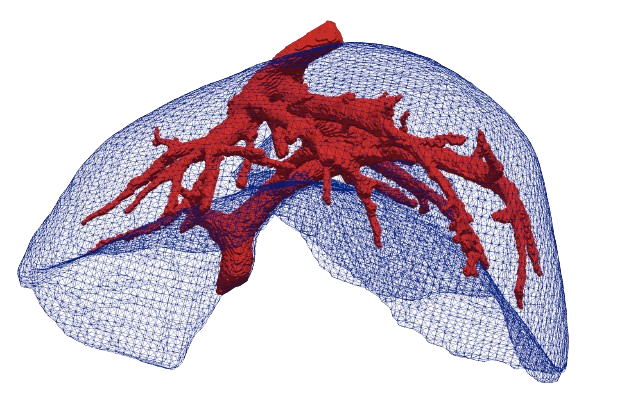
\includegraphics[width=0.95\linewidth]{images/intro/foie.png}
	\end{minipage}
	
	\vspace{3pt}
	\textbf{Current Objective :} Develop hybrid \fcolorbox{red}{white}{finite element} / \fcolorbox{orange}{white}{neural network} methods.
	
	\vspace{1pt}
	\small
	\hspace{150pt} \begin{minipage}{0.14\linewidth}
		\textcolor{red}{accurate}
	\end{minipage} \hspace{10pt} \begin{minipage}{0.3\linewidth}
		\textcolor{orange}{quick + parameterized}
	\end{minipage}

	\vspace{-2pt}

	\normalsize
	\begin{center}
		\begin{tcolorbox}[
			colback=white, % Couleur de fond de la boîte
			colframe=other, % Couleur du cadre de la boîte
			arc=2mm, % Rayon de l'arrondi des coins
			boxrule=0.5pt, % Épaisseur du cadre de la boîte
			breakable, enhanced jigsaw,
			width=0.8\linewidth
			]
			
			\textbf{OFFLINE :}
			
			\begin{figure}[htb]
				\centering
				\resizebox{\textwidth}{!}{%
					\begin{tikzpicture}
						\node at (0,0.8) {Several Geometries};
						\node[draw=none, inner sep=0pt] at (0,0) {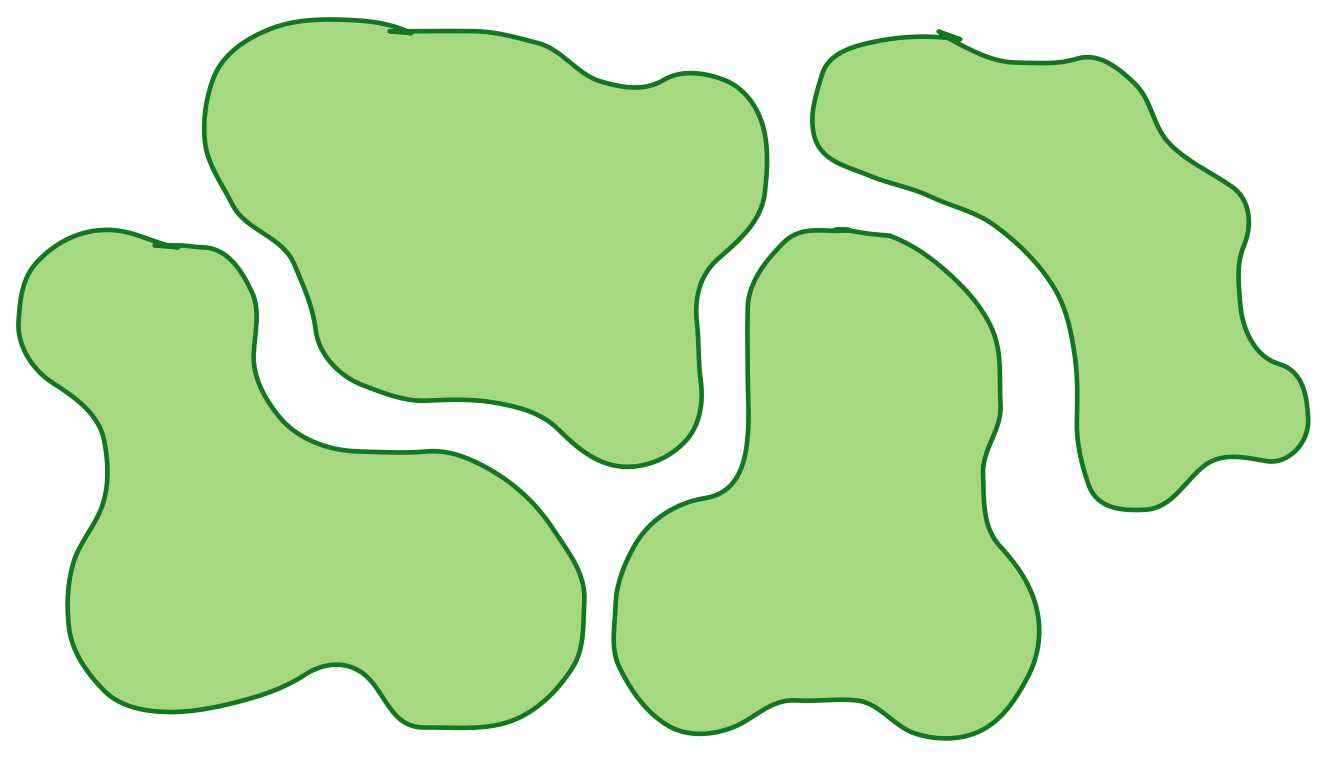
\includegraphics[width=2cm]{images/intro/objective_geom.png}};
						\node[title,font=\Large] at (1.6,0.1) {+};
						\node at (3.5,0.8) {Several Forces};
						\node[draw=none, inner sep=0pt] at (3.5,0) {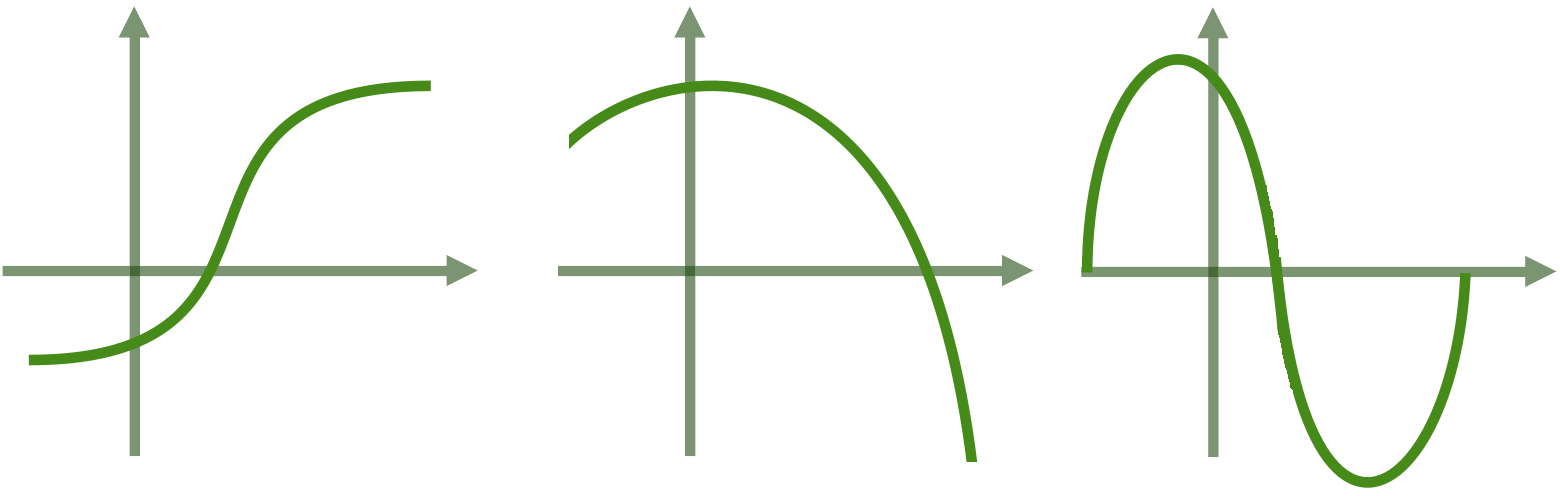
\includegraphics[width=3cm]{images/intro/objective_fct.png}};
						
						% Ajouter une flèche entre les deux rectangles
						\draw[->, title, line width=1.5pt] (5.5,0.1) -- (6.5,0.1);
						%		
						\node at (8,0.8) {Train a PINNs};
						\node[draw=none, inner sep=0pt] at (8,-0.1) {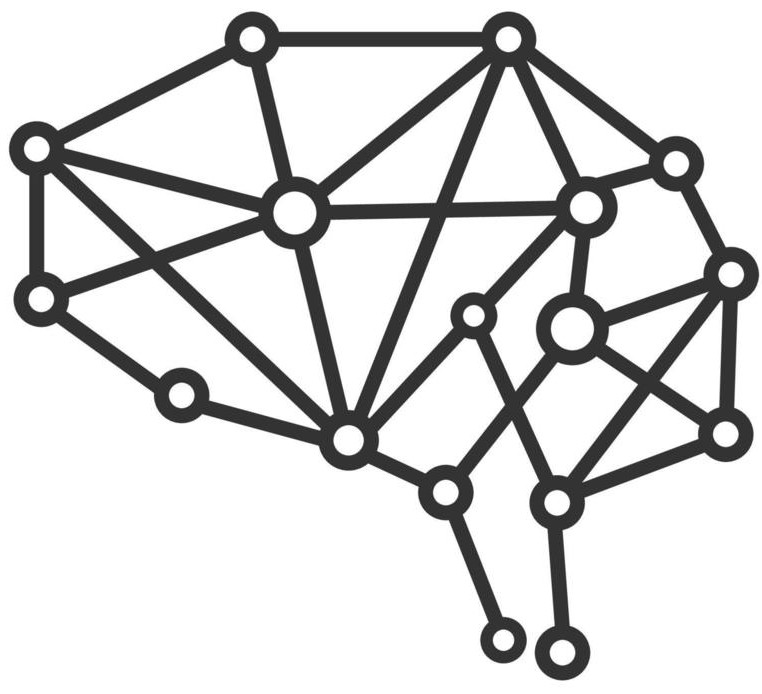
\includegraphics[width=1.5cm]{images/intro/objective_pinns.jpg}};				
					\end{tikzpicture}
				}%
			\end{figure}
			
			\textbf{ONLINE :}
			
			\vspace{-30pt}
			
			\begin{figure}[htb]
				\centering
				\resizebox{\textwidth}{!}{%
					\begin{tikzpicture}
						\node at (0,0.8) {1 Geometry - 1 Force};
						\node[draw=none, inner sep=0pt] at (0,0) {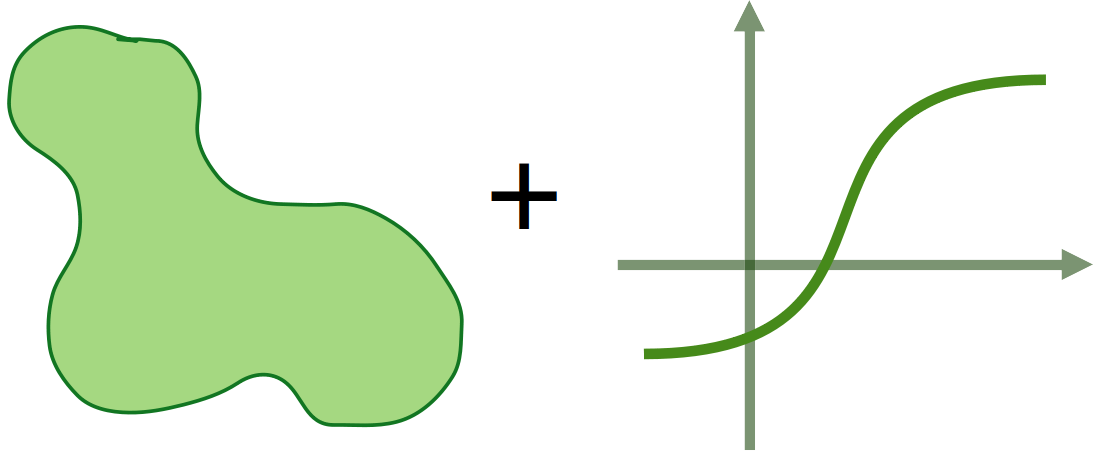
\includegraphics[width=2cm]{images/intro/objective_onegeom_onefct.png}};
						%		\node[title,font=\Large] at (1.6,0.1) {+};
						%		\node at (3.5,0.8) {Several Functions};
						%		\node[draw=none, inner sep=0pt] at (3.5,0) {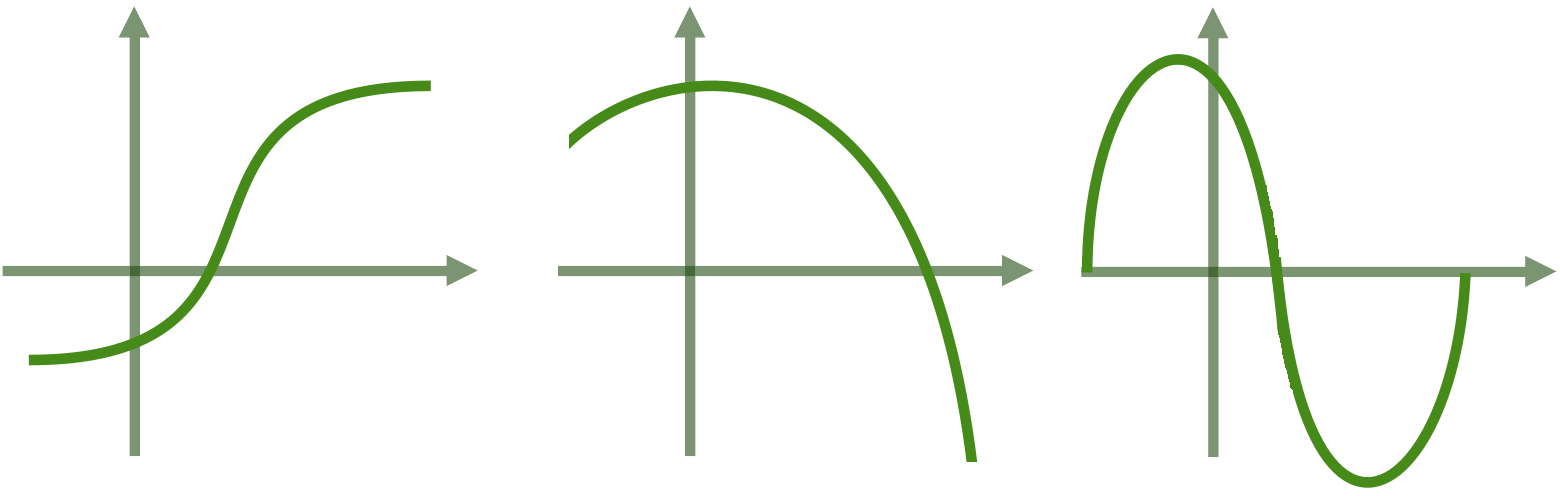
\includegraphics[width=3cm]{images/intro/objective_fct.png}};
						
						\draw[->, title, line width=1.5pt] (2,0.1) -- (3,0.1);
						
						\node[align=center] at (4,1) {Get PINNs \\ prediction};
						\node[draw=none, inner sep=0pt] at (4,-0.1) {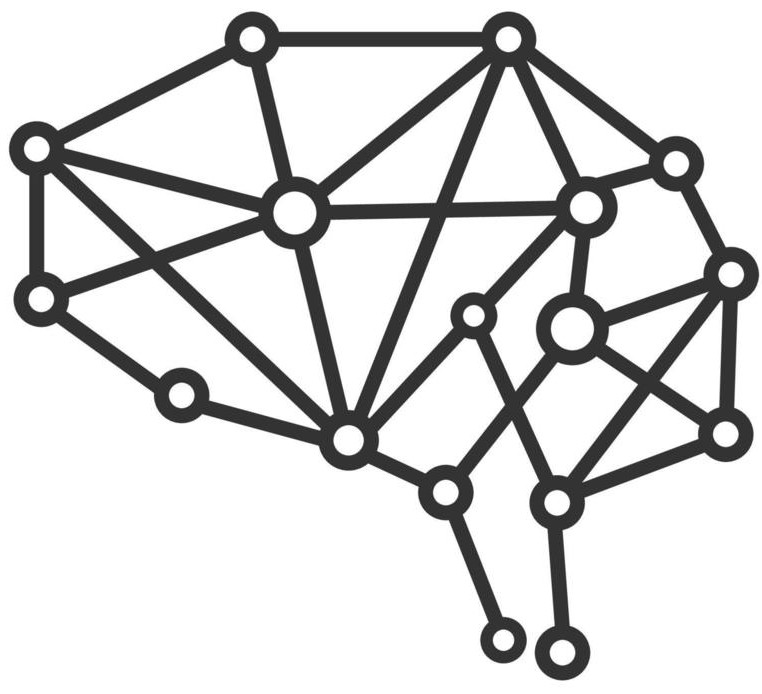
\includegraphics[width=1.5cm]{images/intro/objective_pinns.jpg}};
						
						% Ajouter une flèche entre les deux rectangles
						\draw[->, title, line width=1.5pt] (5.5,0.1) -- (6.4,0.1);
						\draw[draw=black] (6.5,-1) rectangle ++(3,2.5);	
						\node[align=center] at (8,1) {Correct prediction \\ with $\phi$-FEM};
						\node[draw=none, inner sep=0pt] at (8,-0.1) {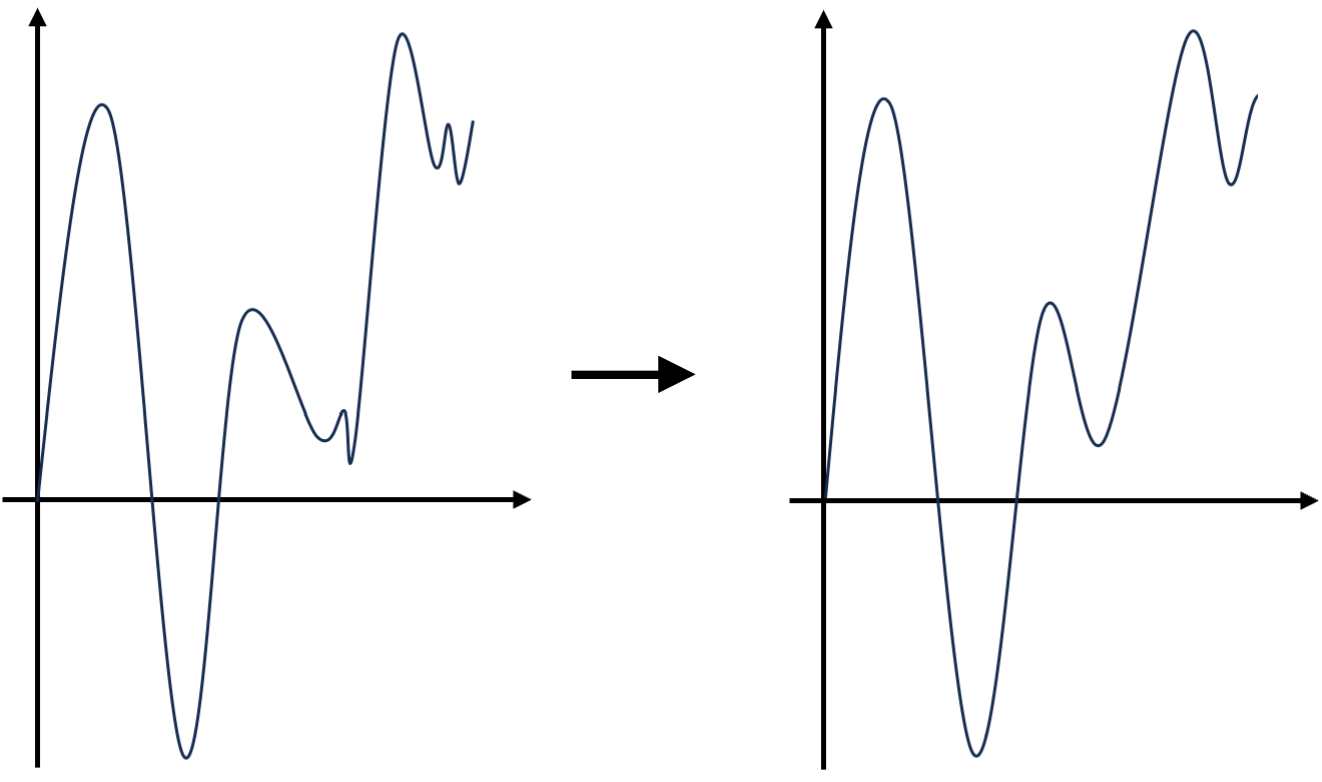
\includegraphics[width=2.5cm]{images/intro/objective_corr.png}};		
					\end{tikzpicture}
				}%
			\end{figure}
		\end{tcolorbox}		
	\end{center}

	\vspace{2pt}
	\textbf{$\phi$-FEM :} New fictitious domain finite element method. \qquad \refappendix{frame:phifem}
	
	$\Rightarrow$ domain given by a level-set function \footnotesize\citep{duprez_phi-fem_2020}\normalsize
\end{frame}

\begin{frame}{Outline}
	\textbf{Two lines of research :}
	
	\begin{enumerate}
		\item How to deal with complex geometry in PINNs ?
		\item Once we have the prediction, how can we improve it (using FEM-type methods) ?
	\end{enumerate}

	\vspace{15pt}

	\textbf{Poisson problem with Dirichlet conditions :} \\
	Find $u : \Omega \rightarrow \mathbb{R}^d (d=1,2,3)$ such that
	\begin{equation}
		\left\{\begin{aligned}
			&-\Delta u(x) = f(x) \quad \text{in } \Omega, \\
			&u(x) = g(x) \quad \text{on } \Gamma
		\end{aligned}\right. \label{edp} \tag{$\mathcal{P}$}
	\end{equation}
	with $\Delta$ the Laplace operator, $\Omega$ a smooth bounded open set and $\Gamma$ its boundary. 
\end{frame}